%DeepL korrigiert
\chapter{Zusammenfassung}

Im Rahmen dieses Kapitels erfolgt zunächst ein Rückblick auf die im Rahmen der Arbeit geleisteten Tätigkeiten sowie eine Zusammenfassung der erzielten Ergebnisse.
Des Weiteren erfolgt eine Evaluierung der Ergebnisse, wobei ein Fazit über die Effektivität und Usability der entwickelten Konzepte gezogen wird.
In diesem Kontext werden ebenfalls Herausforderungen und Schwierigkeiten thematisiert, die bei der Umsetzung der Konzepte entstanden sind.
Abschließend erfolgt ein Ausblick auf potenzielle Weiterentwicklungen der Konzepte.
% DeepL korrigiert

\section{Ergebnisse}

Im Rahmen der Bachelorarbeit wurden zwei Interaktionskonzepte für die Visualisierung von Requirements in Augmented-Reality entwickelt und in jeweils einem Prototyp umgesetzt.
Bei den Prototypen handelt es sich jeweils um eine WebXR-Anwendung, die mit dem Framework Babylon.js in TypeScript entwickelt wurde.
Die Anwendung kann direkt von einem AR-fähigen Browser aufgerufen werden und ist somit plattformunabhängig.

Im ersten Konzept erfolgt die Visualisierung von Requirements in Kombination mit einem möglichst akkuraten 3D-Modell des zu entwickelnden Produkts.
Das 3D-Modell wird vom Nutzer auf einer freien Fläche im Raum platziert und kann in einer Explosionsanimation, welche in Abbildung \ref{fig:porsche-explosion-ar} anhand einer Bildsequenz dargestellt ist, in seine Bauteile zerlegt werden.
Im Rahmen der Zerlegung des Modells werden die Requirements als Panels an den einzelnen Bauteilen visualisiert.
Der Nutzer hat anschließend die Möglichkeit, die Animation wieder rückwärts abzuspielen, um das Modell wieder zusammenzusetzen.
In der Konsequenz werden die Requirements wieder unsichtbar, sodass das Produkt in seinem originalen Gesamtzustand ohne Requirements betrachtet werden kann.
Im Rahmen der Entwicklung des Prototyps wurde ein 3D-Modell eines Fahrzeugs verwendet, welches in einer Animation in seine Einzelteile zerlegt wird.
Zur Veranschaulichung der geplanten Detailansicht besteht im Prototyp die Möglichkeit, die Räder des Modells anzuklicken, um eine Detailansicht der Requirements an die Räder zu erhalten.
Das Interaktionskonzept offenbart ein beachtliches Potenzial, um eine Vielzahl von Interaktionen mit dem 3D-Modell und den Requirements zu ermöglichen.
Ein entscheidender Vorteil der AR-Visualisierung ist die Möglichkeit, das 3D-Modell in Originalgröße darzustellen.
Dadurch wird eine realistische Darstellung des Produkts gewährleistet.
% DeepL korrigiert

\begin{figure}[H]
    \centering
    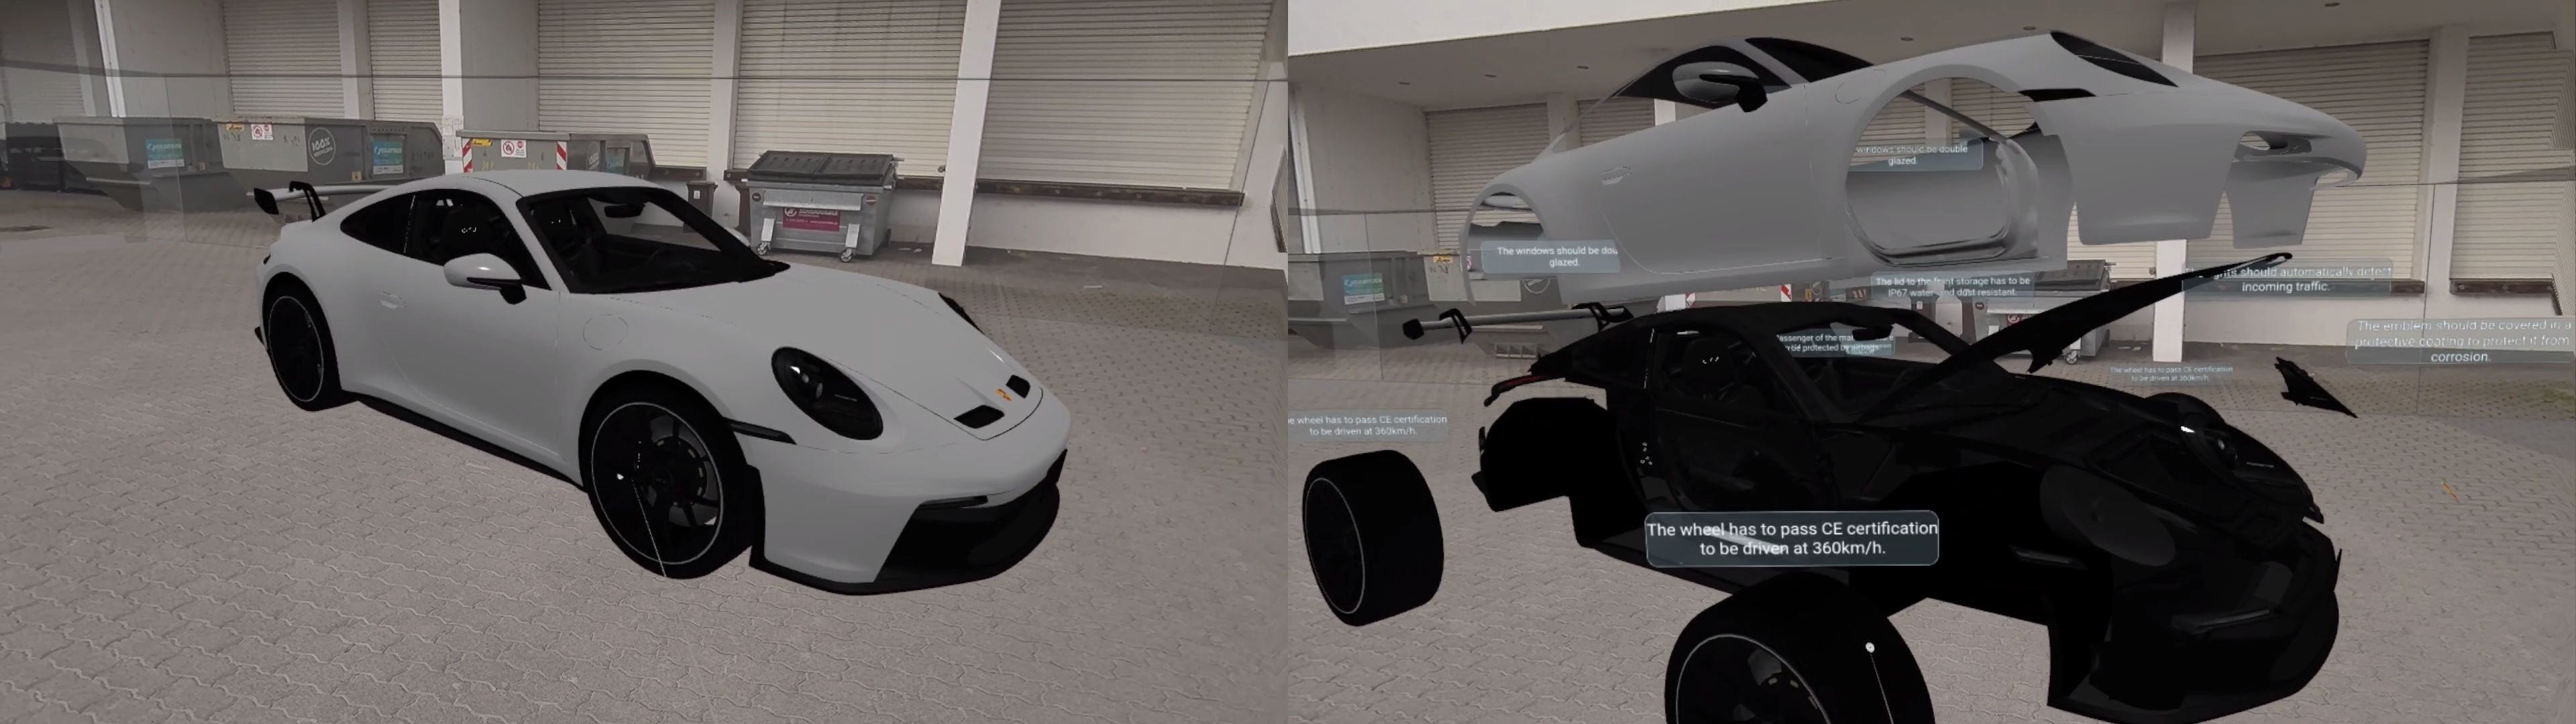
\includegraphics[width=1\textwidth]{images/PorscheExplosionAR.png}
    \caption{Bildsequenz aus dem Prototyp der Explodierenden Bauteile in AR}
    \label{fig:porsche-explosion-ar}
\end{figure}
 
Das zweite Konzept basiert auf der Visualisierung von Requirements in Form von Textpanels, die in der AR-Umgebung schweben.
Die Wolken stellen Cluster aus Requirements dar, die thematisch zusammengehören.
Des Weiteren besteht die Möglichkeit, die Requirements in den Wolken anzuklicken, um zugehörige Requirements anzuzeigen.
Da die Requirements lediglich als Textpanels dargestellt werden, ist die Umsetzung dieses Konzepts deutlich einfacher automatisiert realisierbar, da weder Animationen noch 3D-Modelle erforderlich sind.

Allerdings ist auch der Mehrwert für den Nutzer in diesem Konzept geringer, da es weniger Möglichkeiten zur Interaktion in Augmented-Reality gibt als im ersten Konzept.
Zudem ergeben sich bei der dreidimensionalen Darstellung der Requirementwolken Schwierigkeiten, die in einer zweidimensionalen Darstellung nicht auftreten würden.
Beispielsweise werden Requirements oft hintereinander angezeigt, was dazu führt, dass der Nutzer die Requirements nur schwer oder gar nicht mehr lesen kann.
Auch können nicht sehr viele Requirements in einer Wolke dargestellt werden, da die Requirements sonst zu klein werden und nicht mehr lesbar sind.
In Anbetracht der limitierten AR-spezifischen Interaktionsmöglichkeiten sowie der Herausforderungen bei der Darstellung des Konzepts im dreidimensionalen Raum ist zu hinterfragen, ob das Konzept in AR einen Mehrwert gegenüber einer 2D-Darstellung eines ähnlichen Konzepts bietet.
% DeepL korrigiert


\newpage

\section{Fazit}

Die vorliegende Untersuchung belegt, dass die Visualisierung von Requirements in einer Augmented-Reality-Umgebung zumindest im Rahmen eines Prototyps realisierbar ist.
Das erste Konzept demonstriert zudem, dass durch die Visualisierung in AR mittels diverser neuer Interaktionsmöglichkeiten ein Mehrwert in der Visualisierung von Requirements geschaffen werden kann.

In AR können, wie vor allem am Konzept der explodierten 3D-Modelle gezeigt wurde, viele neue Interaktionsmöglichkeiten geschaffen werden, die in einer 2D-Darstellung nicht möglich wären.
Physische Produkte und ihre Bauteile können in Originalgröße dargestellt und interaktiv mit ihren Requirements verknüpft werden.
So entsteht ein neuer Ansatz, um Requirements besser zu verstehen, zu kommunizieren und zu visualisieren, welcher in anderen Darstellungsformen nur schwer nachzuahmen ist.

Die Untersuchung verdeutlicht jedoch auch, dass die Umsetzung der untersuchten Konzepte noch mit zahlreichen Herausforderungen verbunden ist.
Visuell beeindruckende Darstellungen erfordern in der Regel eine aufwendige und somit kostspielige Implementierung.

Das erste Konzept beispielsweise erfordert die Erstellung und Instandhaltung eines aktuellen 3D-Modells, inklusive Animation des Produkts, welches in der Anwendung dargestellt wird.
Da dieses Konzept der explodierenden Bauteile, welches aber den meisten Mehrwert der Usability bietet, nur schwer automatisiert umzusetzen ist, ist die Implementierung in einer realen Anwendung zeitaufwändig und damit teuer.

Das Konzept der Requirementwolken hingegen ist zwar einfacher umzusetzen, bietet jedoch auch weniger Mehrwert für den Nutzer.
Die Kosten-Nutzen-Effektivität beider Konzepte muss daher in weiteren Untersuchungen genauer betrachtet werden. \newline
Der Vergleich des Konzepts der Requirementwolken in einer dreidimensionalen und zweidimensionalen Darstellung hat gezeigt, dass sich das Konzept der Requirementswolken mehr für eine konventionelle Darstellung in 2D eignet als für eine Implementierung in AR.
Daher sollte das Konzept nicht weiter in AR verfolgt werden.
% DeepL korrigiert

\newpage

\section{Ausblick}
\label{section:ausblick}

In weiteren Forschungsarbeiten könnte die praktische Umsetzbarkeit der beiden Konzepte in einer realen Anwendung weiter untersucht werden.
Eine Untersuchung der professionellen Umsetzbarkeit des Konzepts der explodierenden Bauteile wäre dabei von besonderem Interesse, da dieses bereits im Prototypen den größten Mehrwert der Darstellung bietet und noch signifikant ausgebaut werden kann.
Bei dieser Untersuchung sollte das Konzept vor allem auf Möglichkeiten zur Reduzierung des Aufwands der Implementierung analysiert werden, da die Wirtschaftlichkeit des Konzepts aufgrund der aufwendigen Implementierung noch fraglich ist.


Stellt sich das Konzept als wirtschaftlich sinnvoll heraus, bietet das Konzept vielfältige Möglichkeiten zur Erweiterung der Interaktionen.
Im Folgenden werden einige mögliche Erweiterungen der Interaktionsmöglichkeiten aufgelistet:
\begin{itemize}
    \item Herausgreifen von Bauteilen aus dem explodierten Modell zur genaueren Betrachtung
    \item Rotation ausgewählter Bauteile mit den Joysticks
    \item Manuelle Skalierung von ausgewählten Bauteilen zur genaueren Betrachtung
\end{itemize}

Die im Grundlagenkapitel \ref{sec:gamification-ux} beschriebenen Konzepte der Gamification könnten ebenfalls in die Anwendung integriert werden, um die User Experience zu optimieren.
Dafür könnten beispielsweise bereits betrachtete Bauteile oder Requirements ausgegraut werden, um dem Nutzer eine Übersicht über bereits betrachtete Requirements und ein Gefühl für den \glqq{}Fortschritt\grqq{} in der Betrachtung zu geben.

Das Konzept der Requirementwolken sollte hingegen aufgrund der identifizierten Probleme in 3D als 2D-Darstellung weiter untersucht werden, da sich die Wolken von Requirements auch in einer zweidimensionalen Darstellung realisieren lassen.
In einer 2D-Darstellung könnte das Interaktionskonzept von einer hohen Informationsdichte, wie im Mockup in Kapitel \ref{section:2d} gezeigt, und einer einfachen Navigation der Fläche an Requirements profitieren.
Zudem kann es, wenn es als 2D-Darstellung umgesetzt wird, auch in anderen Anwendungen zur Visualisierung von Requirements eingesetzt werden.
Beispielsweise könnten dafür Erweiterungen für Requirement-Management-Tools wie Jira oder Confluence entwickelt werden, um alternative Visualisierungen als Ergänzung zu den normalen Listen oder Tabellen von Requirements anzubieten.
Dadurch könnte der Kosten-Nutzen-Faktor der Requirementwolken in einer 2D-Darstellung potenziell deutlich verbessert werden.

\newpage

In Abbildung \ref{fig:ausblick-ablauf} sind die nächsten Schritte zur weiteren Untersuchung der beiden Interaktionskonzepte zusammenfassend dargestellt.
Dafür wurden auch mögliche Ziele nächster Untersuchungen definiert, welche auf der hier vorliegenden Arbeit basieren könnten. 

\begin{figure}[H]
    \centering
    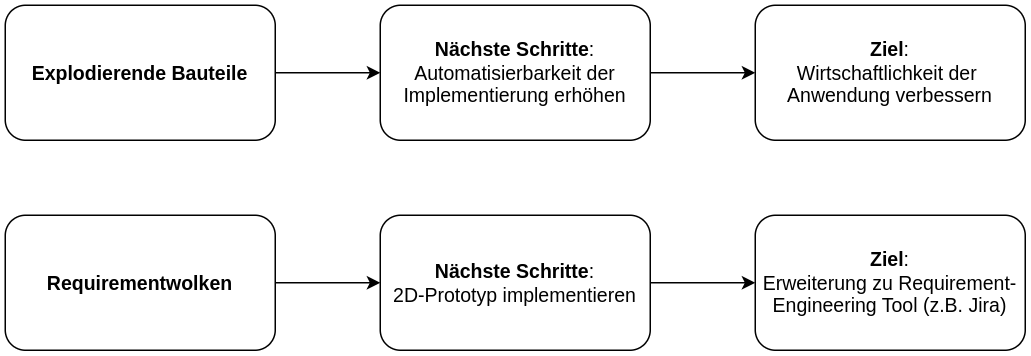
\includegraphics[width=0.9\textwidth]{images/AusblickAblaufdiagramm.png}
    \caption{Ablaufdiagramm der nächsten Schritte zur weiteren Untersuchung der beiden Interaktionskonzepte}
    \label{fig:ausblick-ablauf}
\end{figure}

% DeepL korrigiert